%% FIRE 2026 working note -- NL2PLC shared task
%% Single-column CEUR format (as required by the organizers).
\documentclass{ceurart}

\sloppy

\usepackage{listings}
\usepackage{tikz}
\usetikzlibrary{positioning,arrows.meta,fit,backgrounds}
\graphicspath{{figures/}}

%% Placeholder for the public code repository (to be updated before camera-ready).
\newcommand{\coderepo}{\url{https://github.com/WordsonRobert/AI4Industrial_Automation-FIRE2026}}
%% DOI links in the bibliography resolve through https://doi.org
\providecommand{\doi}[1]{\href{https://doi.org/#1}{\path{#1}}}

\lstdefinestyle{plc}{
  basicstyle=\ttfamily\footnotesize,
  columns=fullflexible,
  keepspaces=true,
  breaklines=true,
  frame=single,
  framerule=0.3pt,
  xleftmargin=2pt,
  xrightmargin=2pt,
  showstringspaces=false,
  keywordstyle=\bfseries,
}
\lstdefinelanguage{ST}{
  morekeywords={PROGRAM,END_PROGRAM,VAR,VAR_INPUT,VAR_OUTPUT,END_VAR,IF,THEN,ELSE,ELSIF,END_IF,AND,OR,NOT,BOOL,INT,TRUE,FALSE,TP,TON,CTU,R_TRIG},
  sensitive=true,
  morecomment=[l]{//},
}

\begin{document}

%% Rights management information. Do NOT modify the footer text below
%% beyond what the organizers specified.
\copyrightyear{2026}
\copyrightclause{Copyright for this paper by its authors.
  Use permitted under Creative Commons License Attribution 4.0
  International (CC BY 4.0).}

\conference{Forum for Information Retrieval Evaluation, December 17--20, 2026, India}

\title{Generating Structured Text and Rust from Natural Language via a Compact Abstract Syntax Tree and Lint-Guided Self-Repair}

\author[1]{Wordson Robert}[%
email=wr24ms190@iiserkol.ac.in,
]
\cormark[1]
\address[1]{Indian Institute of Science Education and Research, Kolkata}

\author[2]{C.Jerin Mahibha}[%
email=jerinmahibha@msec.ac.in,
]
\cormark[1]
\address[2]{Meenakshi Sundararajan Engineering College, Chennai}

\cortext[1]{Corresponding author.}

\begin{abstract}
  We describe our system for the FIRE 2026 NL2PLC shared task, which maps natural language to IEC 61131-3 Structured Text (Task~A) and to Rust (Task~B). A LoRA-tuned Qwen2.5-Coder model (7B or 1.5B) emits a compact JSON abstract syntax tree that a linter and a scan-cycle simulator check; problems are fed back (up to three attempts), and deterministic printers render the tree as Structured Text and Modbus-based Rust. Analysing the 30 submitted test outputs with an independent front-end, interface and timing fidelity measures and 169 behavioural checks derived from the task texts, we find that the 7B model reproduces task interfaces almost perfectly but behaviour poorly: the primary system earns 20 of the 91 checks that require a program to act, and only 2 tasks pass all of their checks. Repair raised verifier-clean programs from 15 to 18 but behavioural credit only from 18 to 20, whereas the 7B model beat the 1.5B model on 9 tasks and lost on none ($p=0.004$), and the Modbus stub, not repair, enables all 18 of 30 Rust compilations.
\end{abstract}

\begin{keywords}
  PLC code generation \sep
  IEC 61131-3 \sep
  Structured Text \sep
  Rust \sep
  LoRA \sep
  self-repair
\end{keywords}

\maketitle

%% =====================================================================
\section{Introduction}
%% =====================================================================

Programmable logic controllers (PLCs) run much of the world's industrial control logic, and their programs are written in the IEC 61131-3 languages~\cite{iec61131-3,john2010iec}, of which Structured Text (ST) is the main textual one. Writing that logic means handling seal-ins, interlocks, timers, counters and edge detection under scan-cycle semantics, where the whole program re-runs every few milliseconds. That makes PLC code a natural but unforgiving target for code LLMs~\cite{chen2021codex,austin2021mbpp,nijkamp2023codegen,li2023starcoder,roziere2023codellama,guo2024deepseekcoder,hui2024qwen25coder}. The FIRE 2026 AI4Industrial Automation task~\cite{fire2026nl2plc} asks systems to turn short specifications, each listing named I/O points with IEC addresses, into ST (Task~A) and Rust (Task~B).

Two properties shaped our design. The setting is extremely low-resource: we had a few hundred examples, and code LLMs perform much worse on rare languages~\cite{cassano2023multiple,cassano2024multiplt}. And many PLC bugs are cheap to detect mechanically: an input never read, an input written to, an output that can never change. We therefore separate \emph{what the program does} from \emph{how it is spelled}. The model writes a compact JSON abstract syntax tree (AST); deterministic code checks that tree, feeds problems back to the model, and prints the result as ST or Rust. Greedy decoding makes our single-pass configuration identical to the first repair attempt, so the effect of repair is directly measurable.

We also analyse the submitted files directly, with an independent ST front-end, interface and timing measures, and behavioural probes. Code, logs and analysis: \coderepo; LoRA adapters on request.

%% =====================================================================
\section{Related Work}
%% =====================================================================

\paragraph{LLMs for PLC code.}
Chat models can produce plausible IEC 61131-3 logic for textbook-style tasks, though it needs expert review~\cite{koziolek2023etfa}; retrieving function-block libraries helps ground it~\cite{koziolek2024rag}. LLM4PLC~\cite{fakih2024llm4plc} closes the loop with a syntax checker, a compiler and a model checker, and Agents4PLC~\cite{liu2024agents4plc} distributes these roles across agents, building on a long tradition of model checking PLC software~\cite{darvas2015plcverif,ovatman2016overview}. We differ in generating an AST rather than text, and in verifying it against the task's own I/O list before printing.

\paragraph{Code LLMs, adaptation and synthetic data.}
Open code models~\cite{nijkamp2023codegen,li2023starcoder,roziere2023codellama,guo2024deepseekcoder,hui2024qwen25coder} are uneven across languages~\cite{cassano2023multiple}, and synthesised data helps low-resource ones~\cite{cassano2024multiplt}. We use LoRA~\cite{hu2022lora}, one of several parameter-efficient methods~\cite{houlsby2019adapters,dettmers2023qlora}, and describe scraped programs with DeepSeek-V3~\cite{deepseekv3}, as in Self-Instruct, Evol-Instruct and OSS-Instruct~\cite{wang2023selfinstruct,luo2024wizardcoder,wei2024magicoder}.
\paragraph{Structured and constrained generation.}
Decoding syntax trees instead of tokens dates to syntactic neural models and abstract syntax networks~\cite{yin2017syntactic,rabinovich2017asn}; with LLMs the same guarantee comes from constrained decoding, via incremental parsing~\cite{scholak2021picard}, constrained semantic decoding~\cite{poesia2022synchromesh}, formal grammars~\cite{geng2023gcd} or token masks~\cite{willard2023outlines}. We do not constrain decoding, and all four of our 7B parse failures are of the kind it prevents (Section~\ref{sec:results}).

\paragraph{Self-repair and verification.}
Self-Debugging, Self-Refine and Reflexion feed execution results or critiques back to the model~\cite{chen2024selfdebug,madaan2023selfrefine,shinn2023reflexion}. Careful studies find the gains modest and limited by feedback quality~\cite{olausson2024selfrepair}, and nearly absent without an external signal~\cite{huang2024cannot}. An alternative is to sample many candidates and select with tests or learned verifiers~\cite{li2022alphacode,chen2023codet,ni2023lever}.
\paragraph{Evaluating code.}
The official metric mixes cosine, structural and program-dependence-graph similarity~\cite{ferrante1987pdg}, akin to CodeBLEU and data-flow-aware models~\cite{ren2020codebleu,guo2021graphcodebert}; such metrics reward similarity to a reference, and even test-based evaluation overstates correctness~\cite{liu2023evalplus}.

%% =====================================================================
\section{Methodology}
%% =====================================================================
For this task we are required to generate Structured Text (ST) and Rust code from natural language descriptions. Our approach is to first generate a compact abstract syntax tree (AST) representation of the given natural-language description of the task using an LLM, and then convert the AST into the required target language using a deterministic printer. We note that the LLM never produces code, but rather an AST representation of the code, which is then deterministically printed. We have a linter and a simulator to check the generated AST for correctness and provide feedback to the LLM for self-repair. Once the AST is verified to be correct, we use a deterministic printer to convert the AST into the required target language (ST or Rust). The overall architecture of our approach along with the preprocessing steps are shown in Figure~\ref{fig:arch}.
\begin{figure}[t]
  \centering
  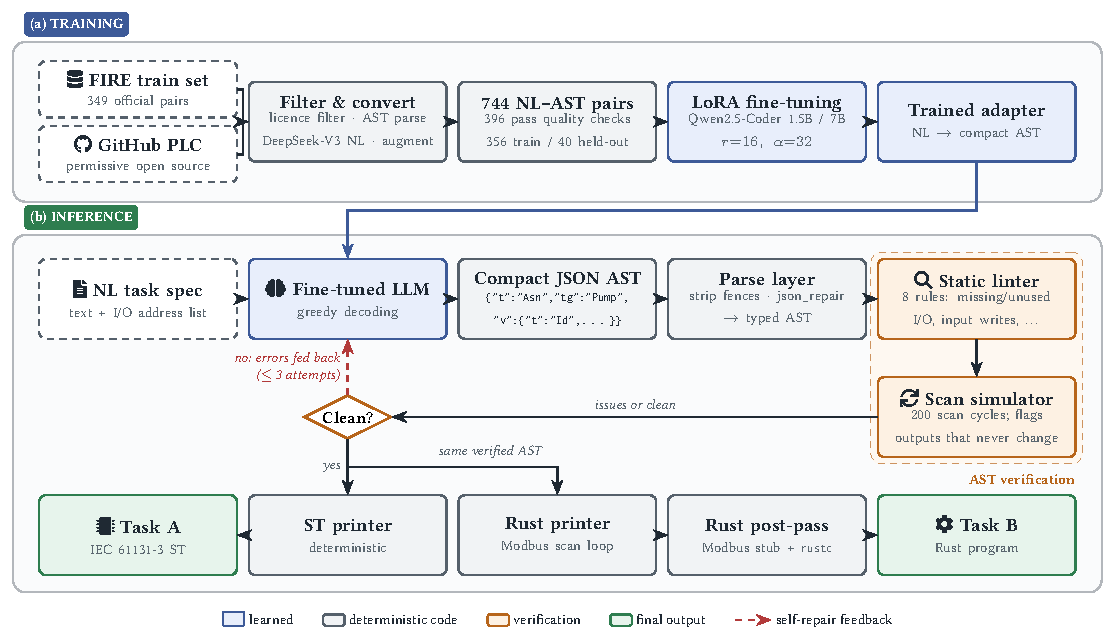
\includegraphics[width=0.86\linewidth]{arch}
  \caption{Overall architecture. (a) LoRA fine-tuning on (NL, compact AST) pairs from the FIRE training set and filtered open-source PLC code. (b) The model emits a compact JSON AST that is parsed, linted and simulated, with up to three attempts; the final AST is printed as ST (Task~A) and Rust (Task~B).}
  \label{fig:arch}
\end{figure}
\subsection{Dataset and Preprocessing}
For the AST generation task, we train Qwen2.5-Coder-7B-Instruct and Qwen2.5-Coder-1.5B-Instruct~\cite{hui2024qwen25coder} with the training data provided by the organizers, together with other permissively licensed open-source PLC projects that we scraped to extend the training corpus.

More concretely, we scraped relevant PLC programs containing IEC 61131-3 Structured Text code licensed under MIT, Apache-2.0, BSD-2-Clause, BSD-3-Clause, ISC, Unlicense, and CC0-1.0 from public GitHub repositories. All accepted PLC program files were first separated into individual program units, after which template and non-program noise was removed. Each program was represented as a structured control/data-flow AST capturing declarations, statements, expressions, function-block calls, and control-flow constructs. Natural-language descriptions were generated for the resulting program units via DeepSeek-V3~\cite{deepseekv3}. The final AST representation contains 18 node types spanning program and variable declarations, assignments, function-block calls, conditional and loop constructs, returns, exits, identifiers, literals, operators, function calls, array indexing, and member access.

\paragraph{Data augmentation and merging.}
To increase variation without requiring additional source programs, accepted programs were augmented through systematic renaming and variable/literal substitution. These transformations preserve the underlying control-logic structure while varying I/O names, tag names, and literal values.

The augmented open-source examples were then combined with the 349 examples in the official FIRE 2026 training set. All examples were converted to the same internal representation before merging, and near-duplicate examples were removed. The resulting corpus contains 744 NL-to-AST training pairs of the form (natural-language specification, compact AST), of which 349 originate from the official FIRE training set and 395 from the additional corpus and augmentation pipeline.

\subsection{LoRA fine-tuning}
We freeze the parameters of the native Qwen2.5-Coder-7B-Instruct and Qwen2.5-Coder-1.5B-Instruct models and attach low-rank adaptation (LoRA)~\cite{hu2022lora} modules to the $q_{proj}$, $k_{proj}$, $v_{proj}$, $o_{proj}$, $gate_{proj}$, $up_{proj}$, and $down_{proj}$ projection layers. We use a LoRA rank of 16, scaling factor $\alpha=32$, and dropout of 0.05, enabling the models to learn the mapping from natural-language PLC specifications to the compact AST representation while keeping the pretrained model parameters fixed.

The 744 total corpus pairs were subject to further quality checks, and the 396 pairs that survived the filtering process were split into 356 training and 40 held-out evaluation examples using a fixed 90/10 split with random seed 42. Training was performed for three epochs using an effective batch size of 16, obtained from a per-device batch size of 1 with 16 gradient-accumulation steps, and a learning rate of $2\times10^{-4}$. We used bfloat16 precision, gradient checkpointing, and a maximum sequence length of 1536 tokens. Training loss and held-out evaluation metrics were monitored throughout training to assess convergence and detect potential overfitting.

\subsection{AST generation and verification}
The fine-tuned model receives a natural-language description of the PLC control task and is prompted to generate the corresponding compact AST in JSON format. The prompt explicitly specifies the AST schema, including the permitted node types and their compact field representations, while constraining the model to output only the JSON AST without explanatory text, Markdown formatting, or Structured Text.

The model uses greedy decoding with a maximum of 2560 newly generated tokens. The generated output is first stripped of Markdown code fences, if present, and parsed as JSON. If standard JSON parsing fails, a JSON-repair procedure is applied before the resulting object is converted into the internal typed AST representation. Outputs that cannot be parsed are marked as generation failures.

The resulting AST is then subjected to two verification stages. First, a rule-based static analyser checks structural and data-flow constraints, including missing required I/O, unused I/O, assignments to input variables, dead overrides, impossible conditions, undeclared variables, and invalid function-block usage. Second, the AST is evaluated using a lightweight PLC scan-cycle simulator to identify dynamic issues such as outputs that remain unchanged during execution. The simulator maintains state across scans and models PLC constructs including timers, counters, and edge detectors.

If either verification stage identifies an issue, the model's previous AST output is appended to the conversation together with a diagnostic feedback message describing the detected issues, and the model is prompted to generate a corrected AST. The process is repeated for up to three attempts, with each iteration consisting of generation, AST parsing, static analysis, and simulation. A clean result terminates the process; otherwise, the last successfully parsed AST is retained.

\subsection{AST to Structured Text conversion}

Following AST generation and verification, the final AST is deterministically
converted into IEC 61131-3 Structured Text (ST) using a dedicated AST-to-ST
printer. The printer traverses the typed AST and generates the corresponding
ST program without further language-model generation. Program declarations are
emitted using a \texttt{PROGRAM} header followed by
\texttt{VAR\_INPUT}, \texttt{VAR\_OUTPUT}, and \texttt{VAR} declaration
blocks as required by the variable scopes represented in the AST. Statements
and expressions are then recursively converted into their corresponding
Structured Text syntax. Parentheses are inserted where necessary to preserve
the precedence of the original expression tree.

The printer also handles formatting and indentation deterministically, with
indentation applied on a per-line basis to maintain valid block structure.
Since the AST retains the original IEC I/O addresses, these addresses remain
available in the intermediate representation during subsequent processing.
\paragraph{Limitations. } In the current implementation, the Structured Text printer does not emit the \texttt{AT} address binding in the generated declaration. For example, a variable represented internally with an address such as
\texttt{\%QX0.0} is printed as \texttt{Fill\_Pump : BOOL;} rather than
\texttt{Fill\_Pump AT \%QX0.0 : BOOL;}. Thus, the generated ST preserves the
variable names and types but does not currently materialize the IEC address
bindings in the output.


\subsection{AST to Rust conversion}

For Task B, the same verified AST is deterministically translated into Rust using a dedicated AST-to-Rust printer. Unlike the AST generation stage, this conversion does not involve further language-model generation. The printer maps the language-independent AST into a Rust program following the execution structure of the FIRE reference implementations, consisting of a Modbus client, a cyclic control loop that reads inputs, evaluates the generated control logic, writes outputs, and pauses for 20~ms between scans. IEC bit-addressed inputs and outputs are mapped to Modbus coils, while word/register addresses are mapped to Modbus holding registers.

The printer translates common PLC function blocks into equivalent Rust state-update logic. In particular, \texttt{TON} timers are represented using scan counters based on the 20~ms scan interval, while \texttt{CTU} and \texttt{R\_TRIG} are also supported. Function blocks not supported by the Rust backend are emitted as comments rather than being fully translated.

\paragraph{Modbus post-processing.}

The generated Rust programs initially reference the external \texttt{modbus} crate. Since the evaluation uses standalone \texttt{rustc} compilation rather than a Cargo-managed dependency environment, these imports would otherwise fail during compilation. The Rust post-processing pass therefore performs a static patching and compilation step. When a generated program contains a Modbus import, the pass prepends a self-contained \texttt{modbus} module implementing an in-memory representation of 256 coils and 256 holding registers, together with the subset of the client interface required by the generated programs. It then checks for missing helper functions, identifies certain dead overrides and hard-coded scan-count timer thresholds, and invokes \texttt{rustc --edition 2021} as a compilation gate.

In the reported runs, the Modbus stub was the only post-processing transformation that actually modified the generated files; the remaining checks were used only for detection and reporting.

\paragraph{Limitations.}

The Rust backend provides only partial coverage of the PLC language and function-block semantics. The current implementation explicitly supports \texttt{TON}, \texttt{CTU}, and \texttt{R\_TRIG}, while other function blocks such as \texttt{TP} and \texttt{TOF} are not fully translated. The printer also uses scan-count approximations for timers and does not implement a complete IEC type system, which can lead to Rust type mismatches during compilation. In addition, certain source constructs and addressing formats remain unsupported, including the \texttt{AI:/DI:} addressing notation present in one test instance.


%% =====================================================================
\section{Results and Discussion}
\label{sec:results}
%% =====================================================================

\paragraph{Configurations and evaluation.}
We compare three submitted configurations on the 30 test tasks: \emph{7B single pass}, \emph{7B + repair} (our primary system) and \emph{1.5B + repair}. With greedy decoding, the single-pass outputs match the first attempt of 7B + repair, so the first pair isolates repair and the second model size. In the official evaluation, which measures similarity to the organisers' reference programs, our team ranked 8th of 8 on Task~A (63.21) and 6th of 7 on Task~B (53.20); as this is one score per team, we analyse the submitted files themselves. Besides the pipeline's verdicts (parseable AST; \emph{clean}: no lint or simulator finding), we measure (i) \emph{front-end validity}: parsing and name resolution by an independent interpreter for the ST subset our printer emits (no type checking), and \texttt{rustc} for Rust; (ii) \emph{interface fidelity}: whether each I/O point of the task's address list is declared under its name, in the correct direction, with an address-consistent type, and is referenced; (iii) whether each stated duration appears as a time literal; and (iv) \emph{behaviour}: per task, an input scenario with checks restricted to behaviour the text states (169 checks; momentary normally open buttons; 20\,ms scan; outputs that are named but not described are not checked), all passed by hand-written reference programs. A program that never drives an output passes 78 checks (every ``stays off'' condition), so we score the other 91 \emph{active} checks and credit one only if the same output also passes every check that requires it to be off; a program that drives every output permanently on passes 50 active checks but earns 2. Active checks fall into \emph{memory} (26: seal-ins, latched faults, hysteresis), \emph{timing} (34: delays, pulses, sequences, counting) and \emph{direct} responses (31). Paired tests are exact McNemar or sign tests over tasks (Table~\ref{tab:results}).

\begin{table}[!tb]
  \caption{Measurements on the 30 test tasks. Interface counts cover the required I/O of parsed programs. $^\dagger$Stub applied post hoc; without it, no printed Rust program compiles.}
  \label{tab:results}
  \centering\small
  \begin{tabular}{lccc}
    \toprule
                                                    & 7B single pass & 7B + repair     & 1.5B + repair \\
    \midrule
    Generation calls / parseable AST                & 30 / 26        & 58 / 27         & 69 / \textbf{30} \\
    Clean (lint and simulation)                     & 15             & \textbf{18}     & 12 \\
    ST passes the front-end check                   & 24             & 25              & 26 \\
    \midrule
    Required I/O declared                           & 120/121        & 125/126         & 140/151 \\
    \quad correct direction / consistent type / referenced & 120 / 116 / 113 & 125 / 121 / 119 & 137 / 133 / 129 \\
    Stated durations present as time literals       & 10/12          & 10/12           & 12/14 \\
    \midrule
    Active checks earned of 91 (tasks passing all checks) & 18 (2)   & \textbf{20} (2) & 4 (0) \\
    \quad memory (26) / timing (34) / direct (31)   & 3 / 3 / 12     & 3 / 3 / 14      & 0 / 1 / 3 \\
    \midrule
    Rust I/O at the Modbus number our mapping prescribes & 113/116   & 118/121         & 137/146 \\
    Rust compiles (\texttt{rustc}, with Modbus stub) & 18$^\dagger$  & 18              & 18 \\
    \bottomrule
  \end{tabular}
\end{table}

\paragraph{The interface is reproduced reliably, the behaviour is not.}
In the parsed 7B programs every required I/O point is declared under its name and in the correct direction, except one that the ST printer dropped (task 4, below), though six are never referenced. 118 of the 121 Rust I/O points of 7B + repair use the Modbus number that the task's address prescribes under our mapping; the only slip drops a digit from all three addresses of task 26 (\texttt{\%IX100.0} becomes \texttt{\%IX10.0}). Behaviour is much weaker. On all 169 checks the three configurations score 77, 78 and 67, against 78 for the program that does nothing; the primary system earns 20 of the 91 active checks, and only tasks 5 and 9 pass all of their checks (Figure~\ref{fig:tasks}). Direct responses succeed most often (14/31), remembered state (3/26) and timing (3/34) rarely; no configuration keeps a hysteresis output in its dead band. Typical failures are start buttons that act only while held (e.g.\ tasks 3, 26), on-delay timers where a pulse or sequence is asked for, and unit errors such as \texttt{T\#10s} for the ``fixed 10 minutes'' of task 17.

\begin{figure}[!tb]
  \centering
  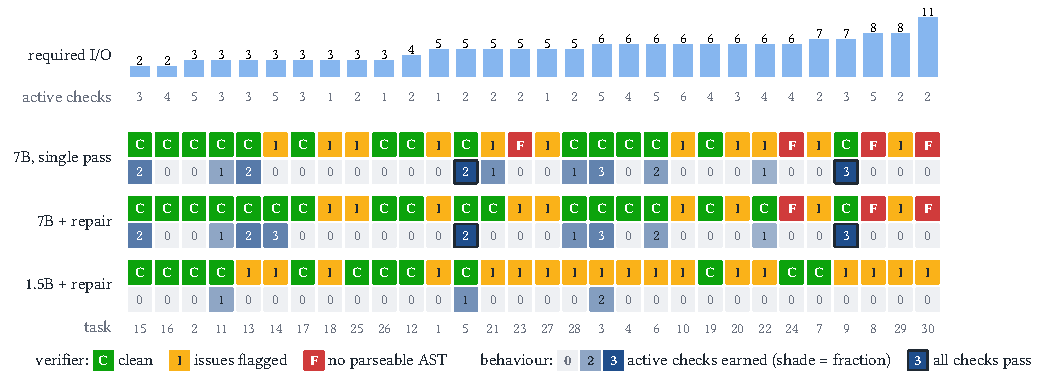
\includegraphics[width=0.9\linewidth]{fig_tasks}
  \caption{Per-task results, sorted by required I/O. Per configuration, the upper row gives the verifier's verdict and the lower row the active checks earned (shade: fraction); outlined cells pass all checks.}
  \label{fig:tasks}
\end{figure}

\paragraph{A clean verdict is a weak indicator of correctness.}
Clean 7B + repair programs earn 33\% of their active checks and flagged ones none: the verdict carries signal, but most clean programs violate the specification. The traffic light of task 2, clean in all configurations, uses pulse timers that all fire at start-up, so all lamps switch on together and stay dark after five seconds. Nor does verification of the tree fully carry over to the printed code: two of the 18 clean ST files fail the front-end check. In task 4 the model gave the counter output a scope label (\texttt{memory}) that the ST printer silently drops, although the Rust printer emits it (the same drop breaks four 1.5B programs and removes five of their required I/O points), and task 21 contains \texttt{IdStop\_Button}, because the model put the node code \texttt{Id} in an operator slot that no lint rule inspects.

\paragraph{Repair fixes what the verifier sees, not the behaviour.}
Repair changed 8 of the 30 7B programs and raised clean programs from 15 to 18 (3 gained, 0 lost; $p=0.25$), but earned checks only from 18 to 20. Its fixes are local (a dead override in task 22, an input write in task 14, a parse failure in task 23), and only task 14 gained behavioural credit. Task 21 lost its credit, showing the loop optimising the verifier rather than the task: to silence an unused-\texttt{Stop\_Button} warning, the model first deleted the button and then added it to the start condition through the invalid operator above. Returns diminish quickly (attempts two and three add 2 and 1 clean 7B programs, 3 and 0 for 1.5B), never-changing 7B outputs stay at nine, and the 1.5B model deletes required I/O to suppress unused-I/O findings (3$\to$6), in line with reports that self-repair is bounded by its feedback~\cite{olausson2024selfrepair,huang2024cannot}.

\paragraph{Model size matters more than repair.}
Against 1.5B + repair, 7B + repair earns more active checks on 9 tasks and fewer on none ($p=0.004$); clean counts point the same way (18 vs.\ 12; $p=0.15$). The 1.5B model always yields a parseable AST, but many of its outputs are on where they should be off: it passes 14 active checks yet earns only 4. It also omits 6 required I/O points, declares 3 in the wrong direction (e.g.\ a position sensor as an output), and misses or mis-binds 9 of 146 Rust I/O points. Of the four 7B parse failures, three are valid JSON drifting towards familiar vocabulary (\texttt{FALSE} as a node type, an invented \texttt{Mod} node, a lowercase \texttt{id}) and one is malformed JSON; constrained decoding prevents all four~\cite{scholak2021picard,poesia2022synchromesh,geng2023gcd,willard2023outlines}. As the configurations fail on different tasks, picking a clean one per task would give 21 clean programs, a simple verifier-based selection~\cite{li2022alphacode,chen2023codet,ni2023lever}.

\paragraph{The Modbus stub, not repair, enables Rust compilation.}
Every printed Rust program imports the external \texttt{modbus} crate, so none compiles standalone; with the 48-line stub 18 do, with or without repair (which gained task 14 and lost task 21). Of the 12 remaining 7B + repair failures, 3 lack an AST, 6 stem from printer gaps (untranslated \texttt{TP} timers and counter outputs, \texttt{MOD}, \texttt{INT}/\texttt{REAL} mixing) and 3 from the model (the invalid operator of task 21; word outputs declared \texttt{BOOL} in tasks 27 and 29). The address analysis also exposes a design error that \texttt{rustc} cannot see: in 24 task statements an input and an output share a number (e.g.\ \texttt{\%IX0.0} and \texttt{\%QX0.0}), and since our printer reads inputs from the coil and holding-register tables instead of the discrete-input and input-register tables~\cite{modbus2012}, each such pair collides on one Modbus address. Finally, the compact AST is 4.2$\times$ longer than the ST it encodes and only 10\% shorter in tokens than a verbose serialisation; its value is checkability, not brevity.

%% =====================================================================
\section{Conclusions and Future Work}
%% =====================================================================

In our system, a LoRA-tuned Qwen2.5-Coder writes only a compact JSON tree that is linted, simulated, repaired and printed as ST and Rust. Measured on the submitted outputs, the 7B model reproduces the task interface almost perfectly (names, directions, types and address numbers of the required I/O) but not behaviour over time: seal-ins, latched faults, hysteresis, delays and sequences account for most failed checks, and only two of thirty tasks pass every behavioural check.

Three lessons follow for LLM-based PLC code generation. First, a verifier that checks structure is a weak proxy for correctness. Clean programs earned only a third of their active checks, and the repair loop, which optimises that verifier, improved the verdict without improving behaviour, and once satisfied a rule in a way that broke the program; repair feedback should therefore come from the specification, not only from generic rules. Second, model capacity mattered more than iteration: the 7B model behaved better than the 1.5B model on 9 tasks and worse on none, although the smaller model always produced a parseable tree. Third, the deterministic components shape the easily measured outcomes, and their defects are the ones the pipeline missed: without the Modbus stub no Rust program compiles, while a dropped variable scope, the missing \texttt{AT} bindings and a shared Modbus address space escaped the linter, the simulator and \texttt{rustc}. Verifying an intermediate representation is only as strong as the guarantee that the printers preserve it.

Our analysis has limitations: the probes are hand-written, cover only stated behaviour and resolve ambiguities by convention (normally open buttons, photo-eyes true when blocked, word outputs carrying the set-point), so they indicate rather than prove correctness; with 30 tasks only large effects are detectable ($p$-values are uncorrected); and the official scores cannot be attributed to configurations.

Future work follows from these findings, in order of expected payoff: (1) derive executable scenarios from the specification, as we did post hoc, and use them as repair feedback and to select among sampled candidates~\cite{chen2023codet,ni2023lever}; (2) make the printers total and checked (emit \texttt{AT} bindings, reject unknown scopes, validate operators, read inputs from the discrete-input and input-register tables, translate \texttt{TP}, \texttt{TOF}, \texttt{CTD} and numeric types in Rust); (3) constrain decoding to the AST schema~\cite{geng2023gcd,willard2023outlines}, which would have prevented all four 7B parse failures; (4) enrich the training data with seal-ins, timers, hysteresis and step sequences, the patterns the models fail on most; and (5) model-check safety properties such as mutually exclusive motor outputs~\cite{darvas2015plcverif,ovatman2016overview}.

\begin{acknowledgments}
  We thank the organizers of the FIRE 2026 AI4Industrial Automation task for the task, the data and their prompt answers, and the authors of the open-source PLC projects in our training corpus.
\end{acknowledgments}

\section*{Declaration on Generative AI}
During the preparation of this work, the author(s) used Claude (Anthropic) to help draft and edit the text of this working note and to help write and debug parts of the pipeline code. After using this tool, the author(s) reviewed and edited the content as needed and take(s) full responsibility for the publication's content. DeepSeek-V3 was used only to generate training descriptions (Section~3.1).

\bibliography{references}

\end{document}
